% this TeX file provides an awesome example of how TeX will make super 
% awesome tables, at the cost of your of what happens when you try to make a
% table that is very complicated.
% Originally turned in for Dr. Nico's Security Class
\documentclass[11pt]{scrartcl}

% Use wide margins, but not quite so wide as fullpage.sty
\marginparwidth 0.5in 
\oddsidemargin 0.25in 
\evensidemargin 0.25in 
\marginparsep 0.25in
\topmargin 0.25in 
\textwidth 6in \textheight 8 in
% That's about enough definitions

% multirow allows you to combine rows in columns
\usepackage{multirow}
% tabularx allows manual tweaking of column width
\usepackage{tabularx}
\usepackage{amsmath}
\usepackage{verbatim}
\usepackage{algorithm}
% packages to include code and highlight it
\usepackage{color}
\usepackage{listings}

\lstset{ %
basicstyle=\footnotesize,       % the size of the fonts that are used for the code
numbers=left,                   % where to put the line-numbers
numberstyle=\footnotesize,      % the size of the fonts that are used for the line-numbers
stepnumber=1,                   % the step between two line-numbers. If it is 1 each line will be numbered
numbersep=5pt,                  % how far the line-numbers are from the code
backgroundcolor=\color{white},  % choose the background color. You must add \usepackage{color}
showspaces=false,               % show spaces adding particular underscores
showstringspaces=false,         % underline spaces within strings
showtabs=false,                 % show tabs within strings adding particular underscores
%frame=single,           % adds a frame around the code
tabsize=2,          % sets default tabsize to 2 spaces
captionpos=b,           % sets the caption-position to bottom
breaklines=true,        % sets automatic line breaking
breakatwhitespace=false,    % sets if automatic breaks should only happen at whitespace
escapeinside={\%*}{*)}          % if you want to add a comment within your code
}

\usepackage[noend]{algpseudocode}
% longtable does better format for tables that span pages
\usepackage{longtable}
\usepackage{graphicx}

\usepackage{hyperref}
\hypersetup{
    colorlinks=true,
    linkcolor=blue,
    filecolor=magenta,      
    urlcolor=red,
    citecolor = black,
}

\begin{document}
% this is an alternate method of creating a title
%\hfill\vbox{\hbox{Gius, Mark}
%       \hbox{Cpe 456, Section 01}  
%       \hbox{Lab 1}    
%       \hbox{\today}}\par
%
%\bigskip
%\centerline{\Large\bf Lab 1: Security Audit}\par
%\bigskip
\author{Alberto Cereser}
\title{Recon3D - a reconstruction software suite for DFXRM}
\subtitle{V. 0.02}
\maketitle

\tableofcontents

\section{Introduction}

Recon3D is a software package to analyze datasets collected using dark-field X-ray microscopy ({\footnotesize{DFXRM}}) {\cite{dfxrm_nat_comm}}, a technique under development at the European Synchrotron Research Facility ({\footnotesize{ESRF}}), beamline {\footnotesize{ID06}}. With {\footnotesize{DFXRM}}, the {\footnotesize{3D}} shape of a deeply embedded grain, and the distribution of the crystallographic orientation inside its volume, is reconstructed from the signal collected in diffraction mode. Data are collected varying three angles: the sample rotation angle $\omega$ and the ``rock'n'roll'' angles $\gamma$ and $\mu$ \cite{henning_joac}. Usually, the same number values, and the same angular increment, is used for the two angles $\gamma$ and $\mu$. 

Recon3D has two main programs, one to load, preprocess and store the collected dataset, and another to reconstruct the sample in {\footnotesize{3D}} (shape and orientation). In detail, the files are:
\begin{itemize}
    \item {\texttt{getdata.py}}, which loads the collected dataset, cleans the images and stores them. In the current version, the software is designed to only reconstruct well-centered grain (see Fig \ref{fig:centered_not_centered})
    \item 
\end{itemize}

\begin{figure}
    \centering
    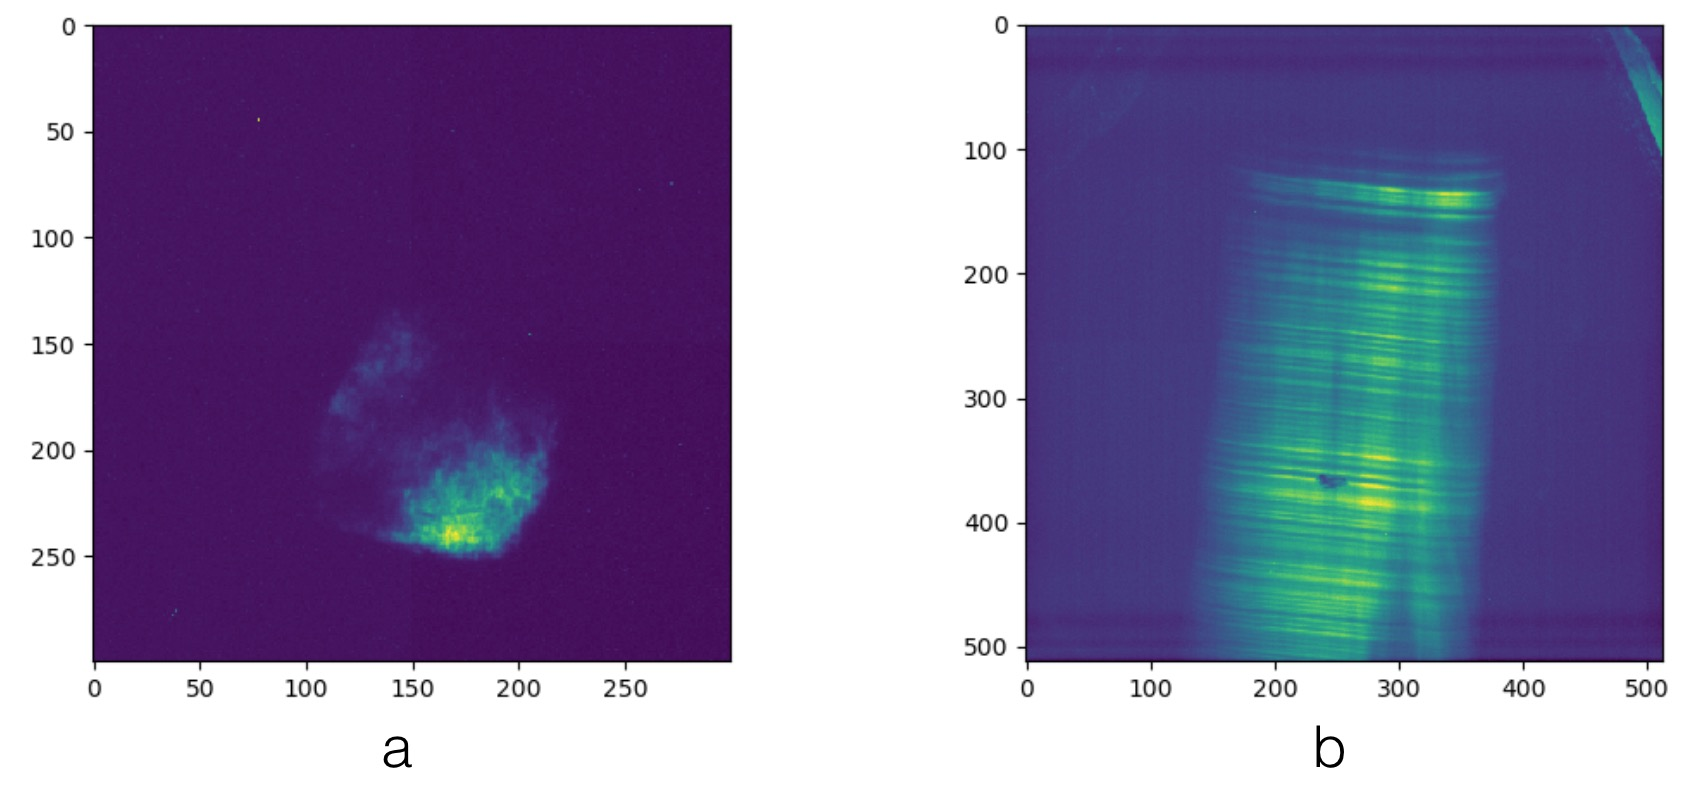
\includegraphics[width=0.75\textwidth]{centered_not_centered}
    \caption{In the current version (v. 0.01), {\texttt{getdata.py}} is designed to take as input frames collected investigating a well centered grain, with the diffraction signal that doesn't touch the borders of the frame, as in {\emph{a}}. The capability to reconstruct samples touching the detector frame ({\emph{b}}) will be later implemented. {\emph{a}} shows a grain in an Al sample (courtesy of Annika Diederichs, {\footnotesize{DTU MEK}}), {\footnotesize{ROI}} size: 300x300; {\emph{b}} shows a crystal in a biomineral sample (courtesy of Phil Cook, {\footnotesize{ESRF}}), {\footnotesize{ROI}} size: 512x512 (entire detector).}
    \label{fig:centered_not_centered}
\end{figure}

\subsection{For developers}

Recon3D is an open source project hosted on \href{https://github.com/albusdemens/Recon3D}{GitHub}. To contribute to the code development, clone\footnote{If you don't know what cloning means, check \href{http://product.hubspot.com/blog/git-and-github-tutorial-for-beginners}{this} introduction to Git and GitHub.} the Recon3D distro and have fun! Except for a few Matlab scripts, all code is written in Python. 

\subsection{Reconstruction steps}

\subsubsection{Data loading, cleaning and storing}

\begin{enumerate}
    \item Have a look at the images using \href{https://sourceforge.net/p/fable/wiki/fabian/}{fabian} or {\texttt{plot\textunderscore img.py}}
    \item If necessary, rebin the data using {\texttt{Rebin\textunderscore img.py}}
    \item Load the collected images using {\texttt{getdata.py}} with 0 as threshold value
    \item Plot the processed images with {\texttt{check\textunderscore threshold.py}}. Look at a few images and select a threshold value. In the next step, all intensities below the threshold value will be set to zero
    \item Look at the distribution of the projection angles. Is there anything anomalous that should be taken into account? Script: {\texttt{Plot\textunderscore angles.py}}
    \item Run {\texttt{getdata.py}}, this time using the threshold value found in the previous step
    \item For each projection, sum all collected images using {\texttt{img\textunderscore sum.py}}
    \item Save each image sum in a separate file using {\texttt{plot\textunderscore sum.py}}
    \item Load the result as a stack in \href{https://imagej.nih.gov/ij/}{ImageJ} or \href{https://imagej.net/Fiji}{\footnotesize{FIJI}}. {\emph{At present, nor ImageJ nor {\footnotesize{FIJI}} are installed on Panda2. Download the data and have a look at the images on your laptop}}
    \item Check how the diffraction projection evolves as the grain rotates. Does the rotation axis move? Are there other grains passing by the detector, as in Fig. \ref{fig:grain_transit}? 
    \item If some projections have to be discarded, change the {\texttt{leno}} loops in {\texttt{getdata.py}}: in this case, we only want to load selected projections. Example: to select projections 1 to 95, 121 to 155 and from 157 to 160, {\texttt{range(leno)}} becomes {\texttt{(range(96) + range(121,156) + range(157, 161))}}. If this is the case, repeat point 5-8
\end{enumerate}
   
\subsubsection{3D reconstruction}    
    
\begin{enumerate}
    \item Calculate the (possible) rotation axis shift using {\texttt{Estimate\textunderscore precession.m}}
    \item Reconstruct the shape of the sample and, for each voxel, calculate the ($\gamma, \mu$) angles for which the maximum intensity was recorded. Code: {\texttt{recon3d.py}}
    \item Convert the output of {\texttt{recon3d.py}} to a {\texttt{vtk}} file, that can be visualized with \href{https://www.paraview.org/}{ParaView}
    \item Play with the {\footnotesize{3D}} reconstruction in ParaView
    \item Compare the reconstructed volume with the experimental data using {\texttt{vol3D.m}}
\end{enumerate}

\begin{figure}
    \centering
    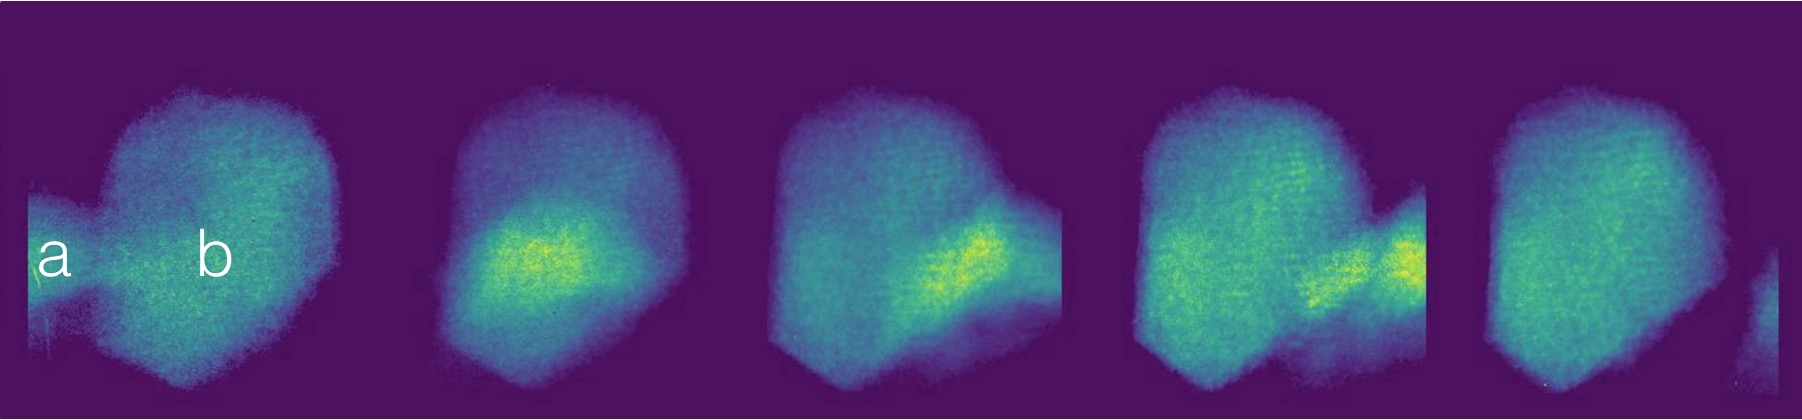
\includegraphics[width=0.9\textwidth]{grain_transit}
    \caption{While scanning grain {\emph{a}} as a function of $\gamma$, $\mu$ and $\omega$, the transit of grain {\emph{b}} was also recorded. This should be avoided.}
    \label{fig:grain_transit}
\end{figure}

To do:
\begin{itemize}
\item List scripts, explain the functioning of each
\item Plot how to use them in a chart
\end{itemize}

\subsection{How to run the scripts}

\subsubsection{check\textunderscore threshold.py}

Script to select which threshold to use to clean the input images with {\texttt{getdata.py}}.

Command: 

{\texttt{\$ python check\textunderscore threshold.py [Data directory] [Modality] [Size frame background subtraction] [Number of projections to consider]}}

\begin{itemize}
    \item {\texttt{Data directory}} is the directory where files returned by {\texttt{getdata.py}} are stored
    \item {\texttt{Modality}}: 1 to show, for each projection, all collected images in an array (like Fig. \ref{fig:img_array}); 2 to show, one by one, all images collected at a certain projection
    \item {\texttt{Number of projections to consider}} defines how many projections to take into account. These are selected by dividing the angular range covered during the tomographic scan in the selected number of steps
\end{itemize}

\subsubsection{estimate\textunderscore precession.m}



\subsubsection{getdata.py}

Script to load the {\texttt{.edf}} files (images and data from header), organize the information and return data in a series of numpy array. Presented in detail in Sec. \ref{sec:getdata}. 

Command:

{\texttt{\$ [mpirun -n NN] python getdata.py [Data directory] [Name data files] [Point of interest] [Image size] [Output path] [Output directory] [Initial phi value] [Initial chi value] [Angular step] [Number of angular steps] [Size frame background subtraction] [Image binarization threshold]}}

Inputs:

\begin{itemize}
    \item {\texttt{mpirun -n NN}} is the command to run the script using parallel computing (multiple processors). The option is available on Panda2. The number of processors to use is {\texttt{NN}}. If mpirun is not available, erase this command
    \item {\texttt{Data directory}} is the directory where data are stored
    \item {\texttt{Name data files}} is the part of the file name that is common to all files (without incremental numbers)
    \item {\texttt{Point of interest}} is the center of the {\footnotesize{ROI}} to consider
    \item {\texttt{Image size}} is the size of the {\footnotesize{ROI}} to consider. Running the reconstruction code on Panda2, the maximum {\footnotesize{ROI}} size is 512$\times$512. If the frames are bigger, rebin them using \ref{sub_s:rebin}
    \item {\texttt{Output path}} is the path where to store the output directory
    \item {\texttt{Output directory}} is the output directory
    \item {\texttt{Initial phi value}} is $\phi_0$ in Eq. \ref{eq:phi}
    \item {\texttt{Initial chi value}} is $\chi_0$ in Eq. \ref{eq:chi}
    \item {\texttt{Angular step}} is the angle, in degrees, used to increment $\chi$ and $\phi$ in the data acquisition script
    \item {\texttt{Number of angular steps}} is the number of considered $\chi$ and $\phi$ increments
    \item {\texttt{Size frame background subtraction}} is the size of the cornice used to clean the image background, to consider possible spatial anisotropies of the detector response. For more details, see {\ref{subs:data_cleaning}}. {\textit{In a future version, the option to reconstruct grains occupying the entire detector frame (no cornice) will be included}}
    \item {\texttt{Image binarization threshold}} is the threshold used to select the diffraction spots and set the outside region to zero. For more details, see {\ref{subs:data_cleaning}}
\end{itemize}

Example: 

{\texttt{\$ python getdata.py /u/data/andcj/hxrm/Al\textunderscore april\textunderscore 2017/ c6\textunderscore topotomo\textunderscore frelon\textunderscore far\textunderscore}} 

{\texttt{256,256 300,300 /u/data/alcer/DFXRM test\textunderscore 2 0.69 -1.625 0.0585 11 20 12}}

\subsubsection{img\textunderscore sum.py}

Sum, for each projection, all images collected by varying $\gamma$ $\mu$. Before saving them, have a look at the summed images and select upper and lower threshold values.

Command: 

{\texttt{\$ python img\textunderscore sum.py [Data directory] [Modality] [Lower threshold] [Upper threshold]}}

\begin{itemize}
    \item {\texttt{Data directory}} is the directory where the output from {\texttt{getdata.py}} is stored
    \item {\texttt{Modality}}: 1 to determine threshold values, 2 to check the rotation axis and 3 to prepare the data for {\footnotesize{ASTRA}}
    \item {\texttt{Lower threshold}} is the possible lower threshold
    \item {\texttt{Upper threshold}} is the possible upper threshold
    
\end{itemize}

\subsubsection{plot\textunderscore angles.py}

Shows the distribution of the $\omega$ angles where the sample was scanned. 

\subsubsection{plot\textunderscore img.py}

Simple script to plot {\texttt{.edf}} files. To show a file, change path in the code. Alternatively, use the \href{https://sourceforge.net/p/fable/wiki/fabian/}{fabian} module included in FabIO \cite{knudsen2013fabio}

\subsubsection{plot\textunderscore sum.py}

Saves the output from {\texttt{img\textunderscore sum.py}} in {\texttt{png}} files. In this way, the sum of all image scollected at a certain projection is saved in a different image. {\textit{Could be included in}} {\texttt{img\textunderscore sum.py}}

\subsubsection{Rebin\textunderscore img.py}
\label{sub_s:rebin}

Script to rebin the topotomo frames, to make the dataset manageable for Panda2. Change paths is the script.

\section{Recommendation for data acquisition}\label{sec:data_acquisition}

\subsection{Data acquisition script}

{\texttt{getdata.py}} is designed to treat data acquired using a macro script structured as follows:

\begin{lstlisting}
def topotomoscan '{

    getinitpos
    
    _omegastart = 0
    _omegaend = 180
    _omegastepsize = 0.8
    _omegasteps = (_omegaend-_omegastart)/_omegastepsize

    for(_omegai = 0; _omegai <= _omegasteps; _omegai += 1){
        
        _omega = _omegastart + _omegai*_omegastepsize
        printf("\n OMEGA = %g\n", _omega)
        umv diffry _omega
        
        _phistepsize = cos(rad(_omega))*0.032
        _chistepsize = sin(rad(_omega))/cos(rad(_zpchi))*0.032
        for(_secondi = 0; _secondi <= 6; _secondi += 1){
            _phi = _zpphi + (_secondi-3)*_phistepsize
            _chi = _zpchi + (_secondi-3)*_chistepsize
            printf("\n chi = %g, phi = %g\n", _chi, _phi)
            umv chi _chi phi _phi
            
            zapline diffrz _zpdiffrz-3.5*0.032 _zpdiffrz+3.5*0.032 7 2000    
        }

    }
    
        
    movetoinit

}'
\end{lstlisting}

In particular, it is important that {\texttt{$_$chistepsize}} and {\texttt{$_$phistepsize}} are described as above (lines 16 and 17). If data have been acquired in the opposite way 

\begin{lstlisting}
        _chistepsize = cos(rad(_omega))*0.032
        _phistepsize = sin(rad(_omega))/cos(rad(_zpphi))*0.032
\end{lstlisting}

In {\texttt{getdata.py}}, function {\texttt{calcGamma(self, data)}} substitute \texttt{self.meta[ind,0]} with \texttt{self.meta[ind,1]}, and \texttt{data.alpha0} with \texttt{data.beta0}.

\section{getdata.py}
\label{sec:getdata}

\begin{figure}[h]
    \centering
    \label{fig:img_array}
    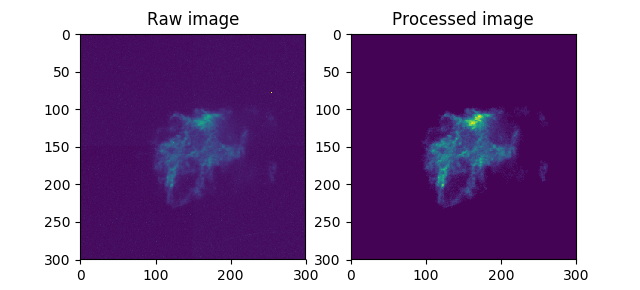
\includegraphics[width=0.9\textwidth]{Raw_processed}
    \caption{Typical dark-field x-ray microscopy ({\footnotesize{DFXRM}}) image before ({\emph{left}}) and after ({\emph{right}}) the data processing procedure here presented.}
    \label{fig:raw_processed}
\end{figure}

{\texttt{getdata.py}} is a script to load, clean and store the {\texttt{.edf}} files collected during to a topotomo scan. The goal of the data cleaning steps is to minimize the noise contribution, enhance the signal from the diffraction spot and normalize the intensity values from different projections.

\subsection{Input data}

\begin{figure}[h!]
    \centering
    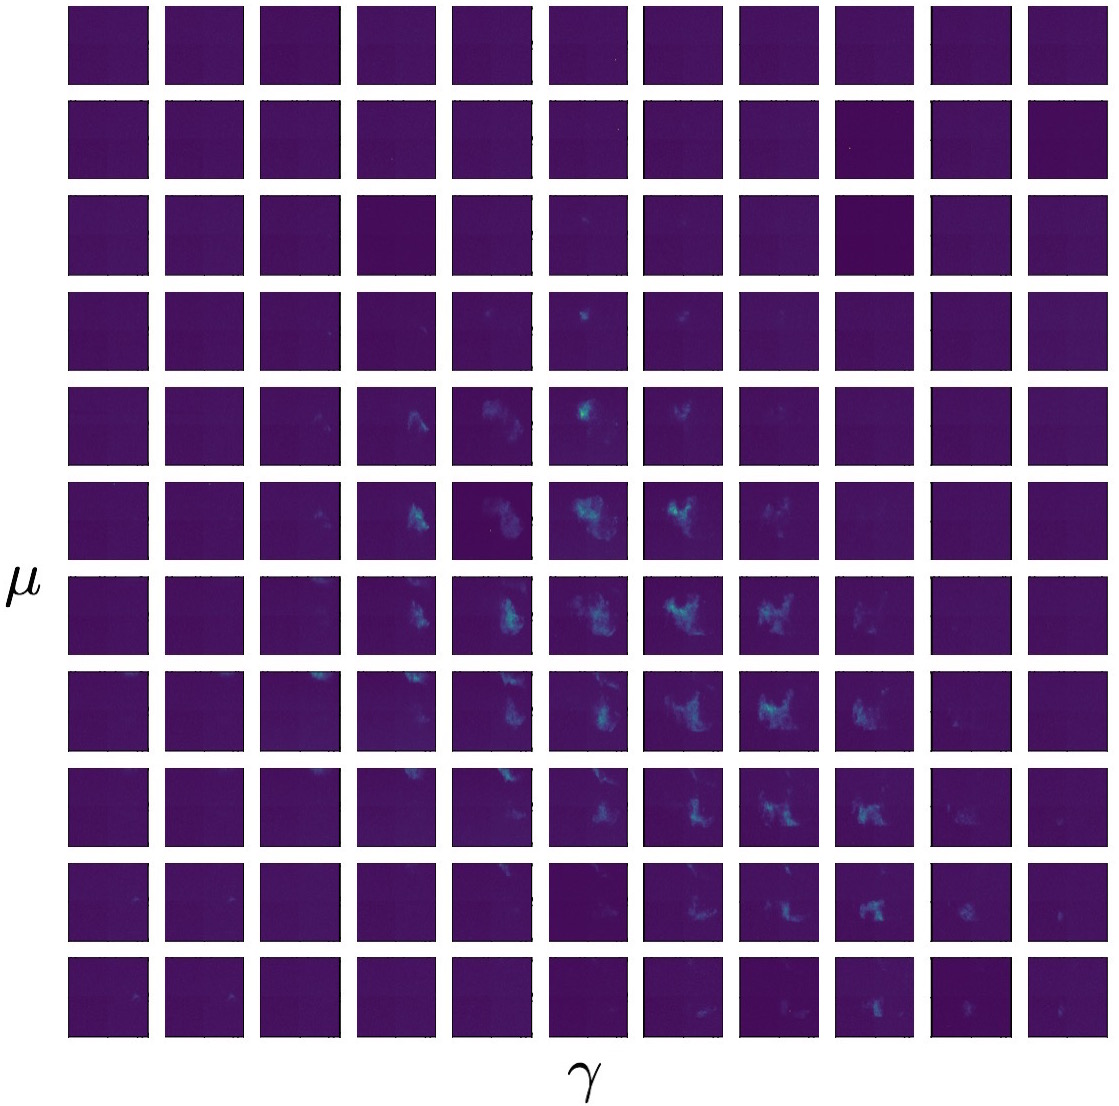
\includegraphics[width=0.85\textwidth]{Img_one_proj}
    \caption{Images collected, at a certain rotation angle $\omega$, by varying the $\gamma$ and $\mu$ angles. For both angles, images were recorded at regular steps with an angular width of 0.0585$^{\circ}$. Sample: deeply embedded grain in a dog-boned Al bar.}
    \label{fig:all_pics_one_om}
\end{figure}

Fig. \ref{fig:all_pics_one_om} shows the frames recorded, at a given projection, varying $\gamma$ and $\mu$ by a constant angular increment ({\emph{topotomo scan}}). From the image, it is evident that the shape of the recorded diffraction spot noticeably changes among frames. This agrees with what expected: for different combinations of $\gamma$ and $\mu$, the Bragg condition is satisfied by different substructures of the considered grain.

As input, {\texttt{getdata.py}} loads a set of images collected during a scan by varying the $\omega, \gamma, \mu$ angles. The images are saved as {\texttt{.edf}} files, each consisting of the actual image and of a header, storing the parameters at which each image has been collected (e.g. motor position, ring current, \ldots) For each image, {\texttt{getdata.py}} reads the header and the image in a five-dimensional matrix: two dimensions are used to store the image, and the other three determine its position in the space of the angles considered during the topo-tomo scan. The angles are:
\begin{itemize}
    \item $\omega$, the sample rotation angle
    \item $\mu$, the in-plane sample tilting angle
    \item $\gamma$, the sample tilting angle perpendicular to $\mu$. The value of $\gamma$ is determined by a {\emph{pseudomotor}}, which is not a real motor but instead a combination of the motors controlling the angles $\chi$ and $\phi$ (a.k.a. $\alpha$ and $\beta$), regulated so that $\gamma$ and $\mu$ always move on two perpendicular planes. In the data acquisition script in Sec. \ref{sec:data_acquisition}, $\chi$ and $\phi$ are defined as 
    
    \begin{eqnarray}
        \phi & = & \phi_0 + i \cdot \Delta \phi \label{eq:phi} \\ 
             & = & \phi_0 + i \cdot \cos\omega \cdot \Delta\gamma \\
        \chi & = & \chi_0 + i \cdot \Delta \chi \label{eq:chi} \\
             & = & \phi_0 + i \cdot \frac{\sin\omega}{\cos\phi_0} \cdot \Delta\gamma
    \end{eqnarray}
    
    From the expression of $\phi$, $\gamma$ can be calculated as 
 
    \begin{equation}
        \gamma = i \Delta\gamma = \frac{\phi - \phi_0}{\cos\omega}
    \end{equation}
    
    To read the header of the {\texttt{.edf}} images, modules from the FabIO\cite{knudsen2013fabio} package were used.
    
\end{itemize}

\subsection{Output}

As output, {\texttt{getdata.py}} generates the following files:

\begin{itemize}
    \item {\texttt{gamma.npy}}, a file listing the values of $\gamma$, a pseudo angle (it's a combination of $\alpha$ and $\beta$, and it's not controlled by a real motor) perpendicular to $\mu$. $\alpha$ and $\beta$ are read from the header of the {\texttt{.edf}} files
    \item {\texttt{mu.npy}}, a file listing all the considered scattering values where frames where collected. Values read from the header of the {\texttt{.edf}} files
    \item {\texttt{omega.npy}}, a file listing, in degrees, the rotation angles where diffraction signal was collected. Values read from the header of the {\texttt{.edf}} files
    \item {\texttt{dataarray.npy}}, a file storing, as a five-dimensional matrix, the coordinates of each diffracted intensity value collected during a topotomo scan. The dimensions are: $\gamma$ angle, $\mu$ angle, $\omega$ angle, X coordinate, Y coordinate. In other words, {\texttt{dataarray.npy}} stores the raw data as a function of the angles where they were collected
    \item {\texttt{cleaning\textunderscore img.npy}}, a file containing, for each considered projection, the frame using to correct for the background current. Dimensions: $\omega$ angle, X coordinate, Y coordinate
    \item {\texttt{dataarray\textunderscore clean.npy}}, a file structured as {\texttt{dataarray.npy}}, containing the collected frames after they have been normalized by the mean, so that the totatl integrated intensity is the same for each projection
    \item {\texttt{dataarray\textunderscore final.npy}}, a file structured as {\texttt{dataarray.npy}}, which contains the frames as they are at the end of the preprocessing procedure
    \item {\texttt{Image\textunderscore properties.txt}}, a text file listing the number of each image and the $\gamma$, $\theta$ and $\omega$ angle where it was collected. $\gamma$, $\theta$ and $\omega$ are read from the header of the {\texttt{.edf}} files
\end{itemize}

\subsection{Data loading}

\subsection{Data cleaning operations}
\label{subs:data_cleaning}

Used nomenclature: {\emph{projection}} is a sample rotation angle where data was acquired; {\emph{frame}} is the image collected at a certain set of $(\omega, \gamma, \mu)$ angles.

\begin{figure}
    \centering
    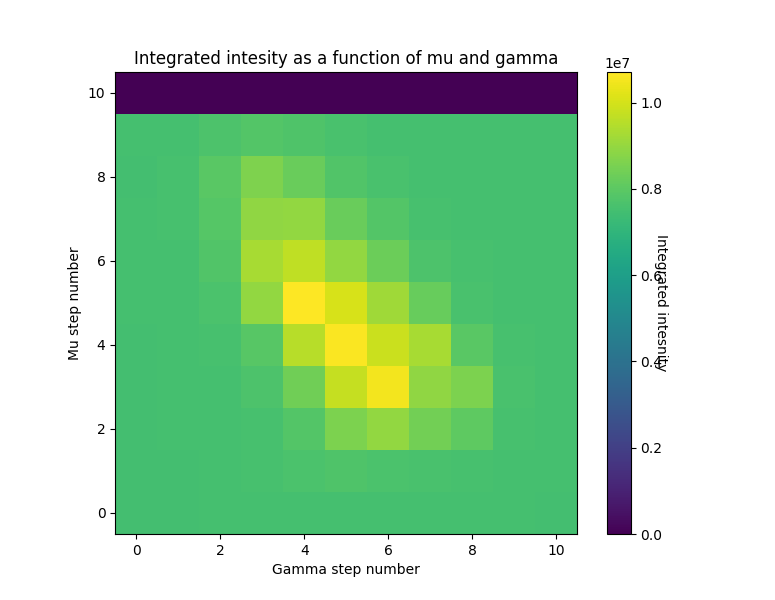
\includegraphics[width=0.62\textwidth]{Distr_I_int}
    \caption{Distribution of the integrated intensity for the frames recorded at a certain projection by varying $\gamma$ and $\mu$. Each pixel represents a different frame. For both $\gamma$ and $\mu$, the step size is 0.0585$^{\circ}$. For a given projection, the first step to clean the recorded frames is to subtract, pixel by pixel, from each frame the average of the two images with the lower integrated intensity.}
    \label{fig:distr_I_int}
\end{figure}

These are the steps followed to clean the collected frames:
\begin{enumerate}
    \item For a given projection, subtract from each frame the dark current (detector readout when there is no incoming signal). The spatial distribution of the dark current on the detector plane is estimated as follows (lines 164-205 in {\texttt{getdata.py}}):
    \begin{enumerate}
        \item Calculate the integrated intensity of each frame (see Fig. \ref{fig:distr_I_int})
        
        \item Select the two frames with the lower (but greater than 0) integrated intensities: $I_{min,1}$ and $I_{min,2}$. If there aren't at least two images with nonzero integrated intensity, define the dark current frame as made of zeros
        
        \item Calculate,pixel by pixel, the average value of $I_{min,1}$ and $I_{min,2}$: $<I_{min}(x,y)> = \frac{I_{min,1}(x,y) + I_{min,2}(x,y)}{2}$. The pixel by pixel operation is designed to take into account possible spatial anisotropies
        
        \item Subtract the dark current frame ($<I_{min}(x,y)>$) from each frame
        
        \item Set negative pixels to 0
        
        \item Threshold hot pixels
    \end{enumerate}
    
    \item Normalize the recorded frames, requiring the total integrated intensity (sum of images collected varying $\gamma$ and $\mu$) to be the same for each projection. In this way, we take into account possible
    variations of the beam power during the experiment, and eventual anisotropies in the sample shape. Steps for a given projection (lines 207-221 in {\texttt{getdata.py}}):
    \begin{enumerate}
        \item Sum all recorded frames
        
        \item Calculate the mean pixel intensity
        
        \item Normalize each frame pixel by pixel dividing by the mean intensity of the relative projection, and multiplying by the mean of all mean values, each relative to a different projection (see Fig. \ref{fig:I_normalization})
            \begin{equation}
                I_{normalized}(x,y)_{\gamma, \mu, \omega} = \frac{I(x,y)_{\gamma, \mu, \omega}}{<\sum_{\gamma, \mu} (x,y)>_{\omega}}\cdot <<\sum_{\gamma, \mu} (x,y)>_{\omega}>
            \end{equation}
    \end{enumerate}
    
    If there are projections where no intensity is recorded, they should be excluded from the calculation of the mean values.
    \begin{figure}[h]
    \centering
    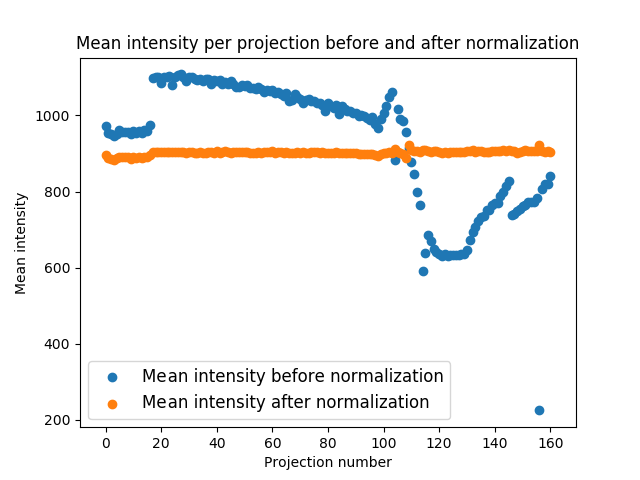
\includegraphics[width=0.75\textwidth]{I_before_after_normalization}
    \caption{Mean pixel intensity per projection before and after normalization.}
    \label{fig:I_normalization}
    \end{figure}
    
    \item For each frame collected in a given projection, characterize the noise distribution and subtract it from the recorded intensity (lines 233-273 in {\texttt{getdata.py}}). Goal: minimize the noise and consider possible spatial anisotropies of the detector response. {\emph{Wolfgang Ludwig suggested that this should not be necessary if the transfocator is managed correctly}}. For a given projection the steps are, as illustrated in Fig. \ref{fig:binning}:
    \begin{enumerate}
        \item Rebin the image (the size of the bin is given as an input when launching {\texttt{getdata.py}})
        
        \begin{figure}[h]
        \centering
        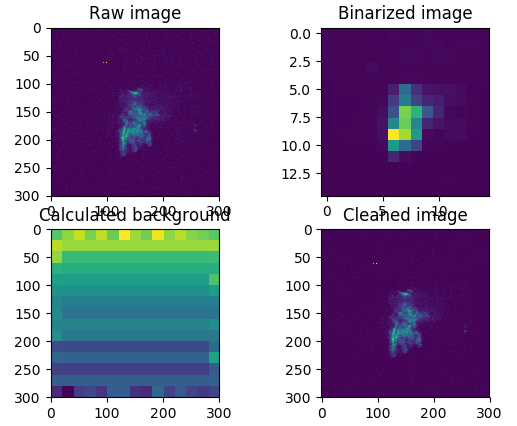
\includegraphics[width=0.75\textwidth]{Background_characterization}
        \caption{Steps used to clean each image from its background signal. After binning (bin size provided as {\texttt{getdata.py}} input), the intensity values of the bins in the cornice, where no diffraction signal is expected, are used to calculate the expected background distribution for the entire image. The background is then subtracted from the image.}
        \label{fig:binning}
        \end{figure}
        
        \item Consider the external cornice (first and last column, first and last row), where normally there is no diffraction signal. {\textbf{This should be changed in case of bad alignment}} 
        
        \item Notice that the background signal tends to progressively increase/decrease along Y
        
        \item Calculate, for each pixel, the relative expected mean background signal using the values of the top and bottom bin from the same column. For a pixel with coordinates $(x,y)$, $IB_{bin,min}$ and $IB_{bin, max}$ are the maximum and minimum intensity of the background signal, calculated considering the top and bottom bins corresponding to the $x$ column. The intensity of the background signal in $(x,y)$, $IB(x,y)$, is then
        \begin{equation}
            IB(x,y) = IB_{bin,min} + \frac{IB_{bin,max} - IB_{bin,min}}{sz(frame) - 2\cdot sz(cornice)}\cdot(y - sz(cornice))
        \end{equation}
        Where $sz(frame)$ and $sz(cornice)$ are the size of the frame and the cornice, respectively
        
        \item Subtract the calculated background from the frame
        
        \item Set to zero all negative pixels
    \end{enumerate}
    
    \begin{figure}
        \centering
        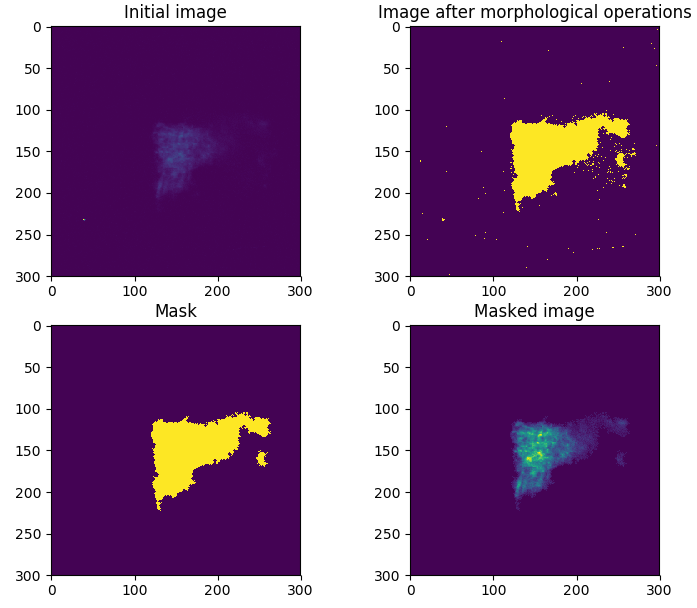
\includegraphics[width=0.75\textwidth]{Morph_ops}
        \caption{The final step of the developed image processing procedure consists in localizing the diffraction spots, and setting to 0 all pixels that are not part of them. This is done by binarizing the image, performing morphological operations, selecting the larger regions and making a mask using them.}
        \label{fig:morph_ops}
    \end{figure}
    
    This procedure can be performed only if the diffraction spot occupies a well defined region at the center of the detector. If that is not the case, set the cornice size to 0. 
    
    \item Localize the regions containing the diffraction signal and set to 0 all pixels outside it (see Fig. \ref{fig:morph_ops}). Lines 274-296 in {\texttt{getdata.py}}. These are the steps in detail:
    \begin{enumerate}
        \item Threshold the input image (threshold value provided as input to {\texttt{getdata.py}}) and binarize the result
        
        \item Fill the holes in the image, and perform the morphological operations of erosion and dilation \cite{image_book}. In Python, a fast and easy way to do so is to use the functions included in \href{http://scikit-image.org/}{skimage} and \href{https://docs.scipy.org/doc/scipy/reference/tutorial/ndimage.html}{ndimage}. Code snippet from {\texttt{getdata.py}}:
        \begin{verbatim}
from skimage.morphology import disk, dilation, erosion
Cleared = ndimage.binary_fill_holes(IM_clean_bin).astype(int)
Dilated = erosion(dilation(Cleared, disk(1)), disk(1))
Dilated_c = ndimage.binary_fill_holes(Dilated).astype(int)
        \end{verbatim}
        
        \item Label the regions in the resulting binary image, and select only those with an area larger than 100 pixels. {\emph{The minimum number of pixels required to consider a cluster as due to a diffraction spot depends on the noise and the signal distribution for a specific sample. A reasonable value should be determined through tests}}
        
        \item Using the selected regions, mask the initial image and set all pixels outside the mask to 0
    \end{enumerate}
    
\end{enumerate}

{\texttt{getdata.py}} also returns an array containing, for each projection, the sum of all collected images. The summed images have been normalized so that they have the same summed intensity. For a given projection {\emph{i}}, the summed image was normalized pixel by pixel using the formula

\begin{equation}
    I_{i,normalized}(x,y) = \frac{I_i(x,y)}{mean(I_i(x,y))} \cdot max\{mean(I_i(x,y))\}_i
\end{equation}

\section{Recon3d.py}

\section{Validation of the shape reconstruction procedure}

\subsection{Validation using ASTRA}

\subsection{Validation using Art + TV}

\section{To dos}

\subsection{Critical}

\begin{enumerate}
    \item In {\texttt{getdata.py}}, include the option to consider the case when the diffraction signal covers the the entire frame, and the cornice methid cannot be used
\end{enumerate}

\subsection{Will make life easier}

\begin{enumerate}
    \item Provide paths as input in 
    \begin{itemize}
        \item {\texttt{Rebin\textunderscore img.py}}
        \item {\texttt{plot\textunderscore img.py}}
        \item {\texttt{plot\textunderscore angles.py}}
    \end{itemize}
    \item Install ImageJ and/or {\footnotesize{FIJI}} on Panda2, to visualize stack of images without the need to download them
    \item Install ParaView on Panda2, to visualize {\footnotesize{3D}} vtk files
    \item Combine {\texttt{img\textunderscore sum.py}} and {\texttt{plot\textunderscore sum.py}}
\end{enumerate}

\subsection{Would be nice to have}

\begin{enumerate}
    \item Adapted version of {\texttt{fabian}} (image visualizer included in FabIO \cite{knudsen2013fabio}) for visualizing sets of {\texttt{.edf}} files. At the moment, {\texttt{fabian}} only works for list of files numbered incrementally. Usually, the images collected during a topotomo scan are named {\texttt{file\textunderscore XXX\textunderscore YYY.edf}}, with {\texttt{YYY}} going from 0 to the number of angular steps (one motor only), and {\texttt{XXX}} increasing by 1 after {\texttt{YYY}} went through all motor values
\end{enumerate}

\section{Code contributors}

In alphabetic order:
\begin{itemize}
    \item Alberto Cereser, contributor 2017
    
    Email: \href{alberto.cereser@gmail.com}{alberto.cereser@gmail.com}, \href{alcer@fysik.dtu.dk}{alcer@fysik.dtu.dk}
    
    Recon3D repository: \href{https://github.com/albusdemens/Recon3D}{https://github.com/albusdemens/Recon3D}

    \item Anders Clemen Jakobsen, contributor 2016/2017
    
    Email: \href{andcj@fysik.dtu.dk}{andcj@fysik.dtu.dk}
    
    Recon3D repository: \href{https://github.com/acjak/Recon3D}{https://github.com/acjak/Recon3D}

\end{itemize}

\bibliographystyle{ieeetr}
\bibliography{Img_cleaning}

\end{document}
